% \section{Qualitative Analysis}
% In this section, we visualize each example from different publication source to compare the articles made by \method~or by human.
% =========================================================================
% Category taxonomy (Definition A): describes the form of the HUMAN baseline
% artifact (not the agent's output). Each case is labeled with the dominant
% output modality (or modalities) of the original human-authored article.
%
%   Visual Artifact      -- Static charts/maps/infographics; core insight is
%                            conveyed through static visualization.
%   Interactive Artifact -- User interaction (hover, click, scrollytelling,
%                            parameter control) is REQUIRED to deliver the
%                            insight. Mere tooltip/decorative hover does NOT
%                            qualify; without the interaction, the insight
%                            must collapse.
%   Video Artifact       -- Contains non-decorative video as a core,
%                            non-substitutable evidence medium.
%   Audio Artifact       -- Contains non-decorative audio as a core,
%                            non-substitutable evidence medium.
%   Textual Artifact     -- Insight is delivered primarily through prose;
%                            charts/photos serve as supporting illustration.
%
% Multi-value rule: a case may carry MORE THAN ONE category when multiple
% modalities are each independently core (removing any of them would break
% the main insight). Multiple values are joined with " + ".
%   Example: "Video + Interactive"
% =========================================================================

\begin{table}[H]
\centering
\small
\renewcommand{\arraystretch}{1.25}
\caption{The Economist: The space race is dominated by new contenders}
\label{tab:caseE1-opening}
\begin{tabularx}{\linewidth}{@{}p{1.8cm} X@{}}
\toprule
\textbf{Data} & {The Great Launch Inversion — 1957 to 2018} \\
\midrule
\textbf{Category} & Audio Artifact + Visual Artifact \\
\midrule
\textbf{Human}~\href{https://www.economist.com/graphic-detail/2018/10/18/the-space-race-is-dominated-by-new-contenders}{[link]} &
Title: \emph{The space race is dominated by new contenders}
\par\smallskip
{\centering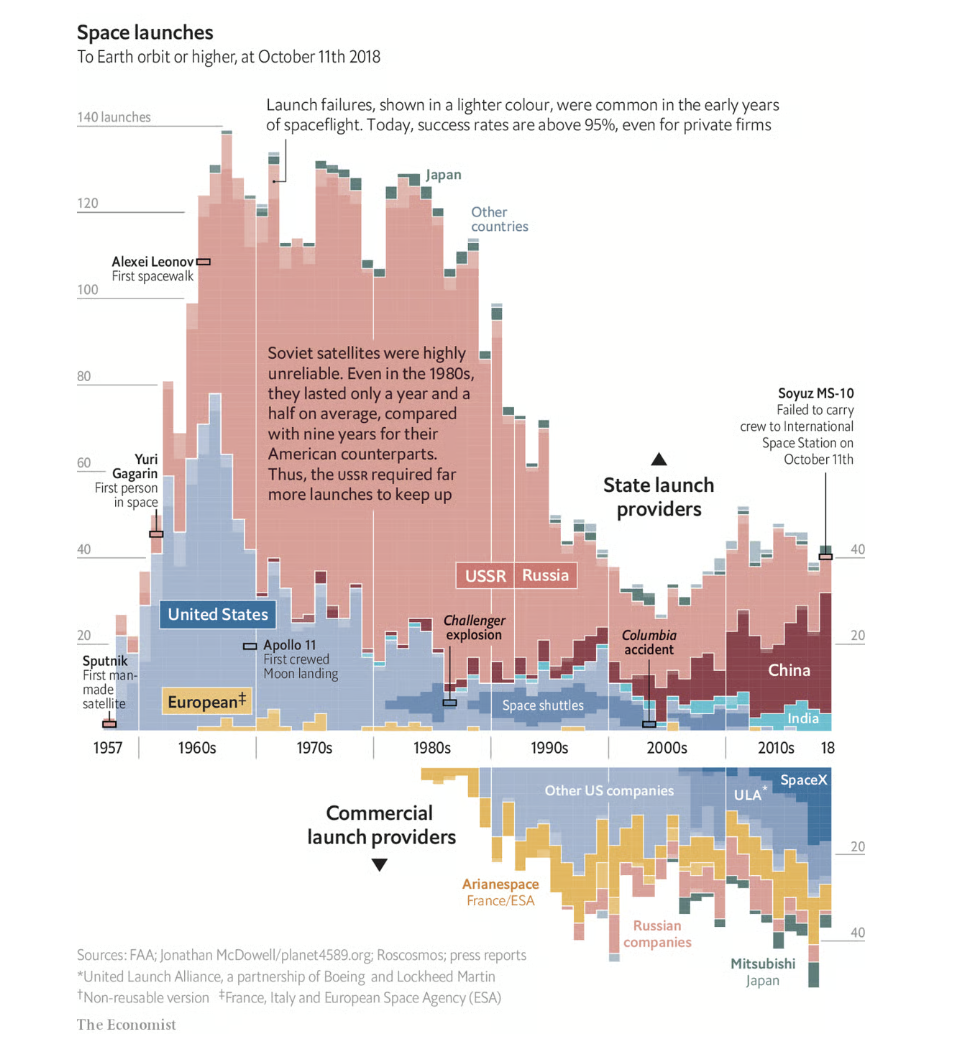
\includegraphics[width=0.5\linewidth]{example/E1/human_chart.png}\par} \\
\midrule
\textbf{Ours}~\href{https://data2story.github.io/economist/01_space-launches/blog_opus47_0503_0236/viewer.html}{[link]} &
Title: \emph{The Great Launch Inversion}
\par\smallskip
{\centering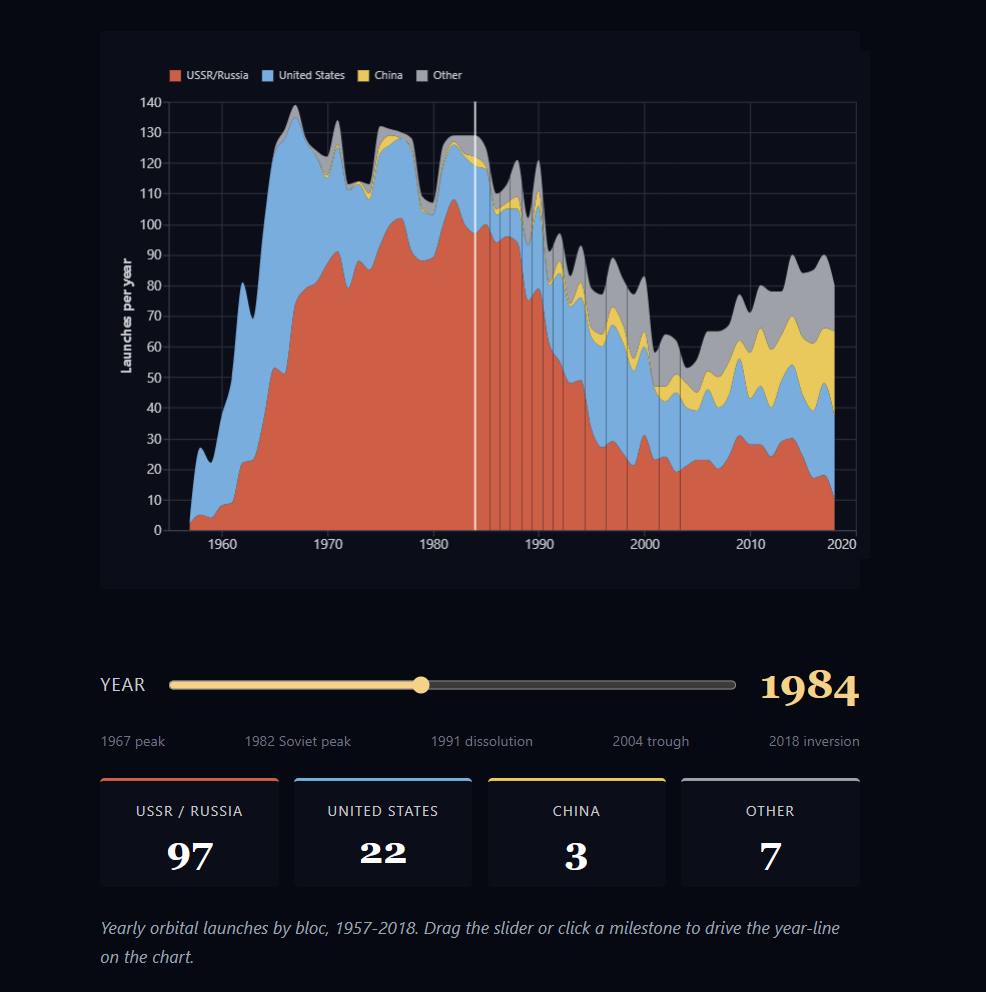
\includegraphics[width=0.5\linewidth]{example/E1/agent_chart.png}\par} \\
\midrule
\textbf{Analyze} &
In the human-written version, a large amount of information is densely packed into a single image. Key moments are annotated with descriptive text, making the chart richer in content and clearer in explanation. In contrast, the agent's version turns the image into an interactive chart, where users can slide along the year axis to view specific numbers for each year. However, it lacks the descriptive annotations found in the human version, so users can only access the raw figures without the surrounding context.
\\
\bottomrule
\end{tabularx}
\end{table}

% \begin{table}[H]
% \centering
% \small
% \renewcommand{\arraystretch}{1.25}
% \caption{The Economist: TV's golden age is real}
% \label{tab:caseE2-opening}
% \begin{tabularx}{\linewidth}{@{}p{1.8cm} X@{}}
% \toprule
% \textbf{Data} & {The Golden Age of TV is real — but it is the floor that rose} \\
% \midrule
% \textbf{Category} & Audio Artifact + Visual Artifact \\
% \midrule
% \textbf{Human}~\href{https://www.economist.com/graphic-detail/2018/11/24/tvs-golden-age-is-real}{[link]} &
% Title: \emph{TV's golden age is real}
% \par\smallskip
% {\centering
\includegraphics[width=0.6\linewidth]{example/E2/human_chart.png}\par}\\
% \midrule
% \textbf{Ours}~\href{https://data2story.github.io/economist/04_tv-ratings/blog_opus47_0503_0238/viewer.html}{[link]} &
% Title: \emph{The Golden Age of TV is real — but it is the floor that rose, not the ceiling.}
% \par\smallskip
% {\centering
% \begin{minipage}[t]{0.48\linewidth}\centering\includegraphics[width=\linewidth]{example/E2/agent_hover_scatter.png}\end{minipage}\hfill
% \begin{minipage}[t]{0.48\linewidth}\centering\includegraphics[width=\linewidth]{example/E2/agent_2.png}\end{minipage}\par} \\
% \midrule
% \textbf{Analyze} &
% The human version packs all the data into a single dense chart, with trend lines, legends, and inline labels marking individual shows directly on the image. The information density is very high and the chart feels crowded, but everything is visible at once. The agent version splits the data across several smaller figures, with far fewer on-chart annotations; details only appear when the user hovers over a specific point.
% \\
% \bottomrule
% \end{tabularx}
% \end{table}

\begin{table}[H]
\centering
\small
\renewcommand{\arraystretch}{1.25}
\caption{The Economist: Managers in football matter much less than most fans think}
\label{tab:caseE3-opening}
\begin{tabularx}{\linewidth}{@{}p{1.8cm} X@{}}
\toprule
\textbf{Data} & {Managers in football matter much less than fans think} \\
\midrule
\textbf{Category} & Audio Artifact + Visual Artifact \\
\midrule
\textbf{Human}~\href{https://www.economist.com/graphic-detail/2019/01/19/managers-in-football-matter-much-less-than-most-fans-think}{[link]} &
Title: \emph{Managers in football matter much less than most fans think}
\par\smallskip
{\centering
\includegraphics[width=0.6\linewidth]{example/E3/human_chart.png}\par} \\
\midrule
\textbf{Ours}~\href{https://data2story.github.io/economist/06_football-managers/blog_opus47_0503_1137/viewer.html}{[link]} &
Title: \emph{Managers in football matter much less than fans think}
\par\smallskip
{\centering
\includegraphics[width=0.6\linewidth]{example/E3/agent_chart.png}\par} \\
\midrule
\textbf{Analyze} &
In the human version, the visualization is clear and well-structured: it shows each manager's expected score, with prominent annotations marking both top-tier players and elite managers. This design makes the fine-grained information immediately readable at a glance. In contrast, the agent blog's chart does not present a clean curve; it reads more like a set of labels positioned along the y-axis of scores. The agent annotates only a few managers but omits the standout players, and the overall distribution is not visually salient.
\\
\bottomrule
\end{tabularx}
\end{table}

% \begin{table}[H]
% \centering
% \small
% \renewcommand{\arraystretch}{1.25}
% \caption{The Economist: Israel's growing settlements force stark choices about its future}
% \label{tab:caseE4-opening}
% \begin{tabularx}{\linewidth}{@{}p{1.8cm} X@{}}
% \toprule
% \textbf{Data} & {The line that quietly crossed — settlements, distance, and arithmetic in the Holy Land} \\
% \midrule
% \textbf{Category} & Audio Artifact + Visual Artifact \\
% \midrule
% \textbf{Human}~\href{https://www.economist.com/graphic-detail/2019/02/02/israels-growing-settlements-force-stark-choices-about-its-future}{[link]} &
% Title: \emph{Israel's growing settlements force stark choices about its future}
% \par\smallskip
% {\centering
\includegraphics[width=0.6\linewidth]{example/E4/human_chart.png}\par} \\
% \midrule
% \textbf{Ours}~\href{https://data2story.github.io/economist/07_holy-land/blog_opus47_0503_1155/viewer.html}{[link]} &
% Title: \emph{The line that quietly crossed}
% \par\smallskip
% {\centering
\includegraphics[width=0.6\linewidth]{example/E4/agent_chart.png}\par} \\
% \midrule
% \textbf{Analyze} &
% The human chart casts the problem as a triangle: three policy goals sit at the vertices and three mutually exclusive outcomes sit on the edges, making the three-way trade-off readable at a glance. The agent version reduces the same problem to a single time series of the Jewish population share with a 50\% reference line. The trend is accurate, but it captures only one of the three constraints, and the relational structure that gives the human chart its analytical power is lost.
% \\
% \bottomrule
% \end{tabularx}
% \end{table}

% \begin{table}[H]
% \centering
% \small
% \renewcommand{\arraystretch}{1.25}
% \caption{The Economist: The Oscars' influence has waned}
% \label{tab:caseE5-opening}
% \begin{tabularx}{\linewidth}{@{}p{1.8cm} X@{}}
% \toprule
% \textbf{Data} & {Best Picture, Forgotten Picture} \\
% \midrule
% \textbf{Category} & Audio Artifact + Visual Artifact \\
% \midrule
% \textbf{Human}~\href{https://www.economist.com/graphic-detail/2019/03/02/the-oscars-influence-has-waned}{[link]} &
% Title: \emph{The Oscars' influence has waned}
% \par\smallskip
% {\centering
\includegraphics[width=0.6\linewidth]{example/E5/human_chart.png}\par} \\
% \midrule
% \textbf{Ours}~\href{https://data2story.github.io/economist/09_oscars-influence/blog_opus47_0503_1157/viewer.html}{[link]} &
% Title: \emph{Best Picture, Forgotten Picture}
% \par\smallskip
% {\centering
\includegraphics[width=0.6\linewidth]{example/E5/agent_chart.png}\par} \\
% \midrule
% \textbf{Analyze} &
% The human chart is a single dense ranked list of films sorted by share of references, with Best Picture winners and nominees color-coded inline. Every row is visible at once, so the reader can scan the full distribution and find any specific film directly, though the view is static and non-interactive. The agent reframes the same dataset as a year-by-year comparison between the Academy Pick and the People's Pick, exposed through a draggable year selector. It surfaces the gap one year at a time but hides the global ranking.
% \\
% \bottomrule
% \end{tabularx}
% \end{table}

% \begin{table}[H]
% \centering
% \small
% \renewcommand{\arraystretch}{1.25}
% \caption{The Economist: Tourism flows and death rates suggest covid-19 is being under-reported}
% \label{tab:caseE6-opening}
% \begin{tabularx}{\linewidth}{@{}p{1.8cm} X@{}}
% \toprule
% \textbf{Data} & {A map that already lied — Tracking the stealthy killer, March 2020} \\
% \midrule
% \textbf{Category} & Audio Artifact + Visual Artifact \\
% \midrule
% \textbf{Human}~\href{https://www.economist.com/graphic-detail/2020/03/07/tourism-flows-and-death-rates-suggest-covid-19-is-being-under-reported}{[link]} &
% Title: \emph{Tourism flows and death rates suggest covid-19 is being under-reported}
% \par\smallskip
% {\centering
\includegraphics[width=0.6\linewidth]{example/E6/human_chart.png}\par} \\
% \midrule
% \textbf{Ours}~\href{https://data2story.github.io/economist/13_covid19/blog_opus47_0503_1207/viewer.html}{[link]} &
% Title: \emph{A map that already lied.}
% \par\smallskip
% {\centering
\includegraphics[width=0.6\linewidth]{example/E6/agent_chart.png}\par} \\
% \midrule
% \textbf{Analyze} &
% The human chart uses a stacked daily-share time series from late January to early March 2020, with countries layered as colored bands. The reader can see how the relative share of each country evolves day by day, and the cross-country shift of the outbreak from China to the rest of the world is directly visible. The agent reduces the same dataset to a snapshot of confirmed cases on a single day, shown as a log-scale ranking. Magnitudes are precise, but the temporal dynamic is lost.
% \\
% \bottomrule
% \end{tabularx}
% \end{table}

\begin{table}[H]
\centering
\small
\renewcommand{\arraystretch}{1.25}
\caption{The Pudding: The Structure of Stand-Up Comedy}
\label{tab:caseP1-opening}
\begin{tabularx}{\linewidth}{@{}p{1.8cm} X@{}}
\toprule
\textbf{Data} & One Ten-Second Laugh — The Architecture of Ali Wong's Baby Cobra \\
\midrule
\textbf{Category} & Video Artifact + Interactive Artifact \\
\midrule
\textbf{Human}~\href{https://pudding.cool/2018/02/stand-up/}{[link]} &
Title: \emph{The Structure of Stand-Up Comedy}
\par\smallskip
{\centering
\includegraphics[width=0.6\linewidth]{example/P1/human_chart.png}\par} \\
\midrule
\textbf{Ours}~\href{https://data2story.github.io/pudding/02_stand-up/blog_opus47_0503_0049/viewer.html}{[link]} &
Title: \emph{One ten-second laugh, and what holds it up}
\par\smallskip
{\centering
\includegraphics[width=0.6\linewidth]{example/P1/agent_chart.png}\par} \\
\midrule
\textbf{Analyze} &
In the human-authored version, the video is embedded inline within the dense surrounding text and plays automatically, with a live transcript animating alongside the playback. The effect is polished and attention-holding, reflecting careful design work. The agent-generated version, by contrast, simply embeds a static YouTube iframe that requires the reader to click through and watch the video on YouTube itself.
\\
\bottomrule
\end{tabularx}
\end{table}

% \begin{table}[H]
% \centering
% \small
% \renewcommand{\arraystretch}{1.25}
% \caption{The Pudding: Are Men Singing Higher in Pop Music?}
% \label{tab:caseP2-opening}
% \begin{tabularx}{\linewidth}{@{}p{1.8cm} X@{}}
% \toprule
% \textbf{Data} & {The Top of the Charts Sang Higher in 2019 Than in Any Year Since 1958} \\
% \midrule
% \textbf{Category} & Video Artifact + Interactive Artifact\\
% \midrule
% \textbf{Human}~\href{https://pudding.cool/2019/08/register/}{[link]} &
% Title: \emph{Are Men Singing Higher in Pop Music?}
% \par\smallskip
% {\centering
\includegraphics[width=0.6\linewidth]{example/P2/human_chart.png}\par} \\
% \midrule
% \textbf{Ours}~\href{https://data2story.github.io/pudding/06_register/blog_opus47_0503_0049/viewer.html}{[link]} &
% Title: \emph{The top of the charts sang higher in 2019 than in any year since 1958.}
% \par\smallskip
% {\centering
\includegraphics[width=0.6\linewidth]{example/P2/agent_chart.png}\par} \\
% \midrule
% \textbf{Analyze} &
% The human chart overlays the time series with a translucent portrait of a 1980s rock vocalist, anchoring the 1988 peak in cultural memory and using a bold annotation and a single highlighted point to direct the eye. The agent version strips away the editorial atmosphere and emphasizes quantitative comparison: the historical peak and the new record are each marked with an explicit value, so the half-point gap between them is immediately legible without relying on prior context.
% \\
% \bottomrule
% \end{tabularx}
% \end{table}

% \begin{table}[H]
% \centering
% \small
% \renewcommand{\arraystretch}{1.25}
% \caption{The Pudding: They Won't Play a Lady-O on Country Radio}
% \label{tab:caseP3-opening}
% \begin{tabularx}{\linewidth}{@{}p{1.8cm} X@{}}
% \toprule
% \textbf{Data} & {The Silence Between the Songs — Country Radio in 2022} \\
% \midrule
% \textbf{Category} & Interactive Artifact \\
% \midrule
% \textbf{Human}~\href{https://pudding.cool/2023/05/country-radio/}{[link]} &
% Title: \emph{They Won't Play a Lady-O on Country Radio}
% \par\smallskip
% {\centering
\includegraphics[width=0.6\linewidth]{example/P3/human_chart.png}\par} \\
% \midrule
% \textbf{Ours}~\href{https://data2story.github.io/pudding/09_country-radio/blog_opus47_0503_0049/viewer.html}{[link]} &
% Title: \emph{They Won't Play a Lady-O on Country Radio}
% \par\smallskip
% {\centering
\includegraphics[width=0.6\linewidth]{example/P3/agent_chart.png}\par} \\
% \midrule
% \textbf{Analyze} &
% The human chart resolves the data at the daypart level, exposing the surprising concentration of back-to-back plays in the overnight window and revealing the full distribution across five time windows. The agent version collapses the same data into a binary graveyard-versus-prime split, which sharpens the editorial framing of unequal airtime but discards the within-period structure. The human design rewards a close reading of when the back-to-backs occur; the agent design optimizes for an at-a-glance asymmetry.
% \\
% \bottomrule
% \end{tabularx}
% \end{table}

\begin{table}[H]
\centering
\small
\renewcommand{\arraystretch}{1.25}
\caption{The Pudding: Internet Boy Band Database}
\label{tab:caseP4-opening}
\begin{tabularx}{\linewidth}{@{}p{1.8cm} X@{}}
\toprule
\textbf{Data} & {The look you remember is one of four — Boy bands, by the data} \\
\midrule
\textbf{Category} & Audio Artifact + Interactive Artifact \\
\midrule
\textbf{Human}~\href{https://pudding.cool/2018/11/boy-bands/}{[link]} &
Title: \emph{Internet Boy Band Database}
\par\smallskip
{\centering
\includegraphics[width=0.6\linewidth]{example/P4/human_chart.png}\par} \\
\midrule
\textbf{Ours}~\href{https://data2story.github.io/pudding/12_boybands/blog_opus47_0503_0109/viewer.html}{[link]} &
Title: \emph{The look you remember is one of four}
\par\smallskip
{\centering
\includegraphics[width=0.6\linewidth]{example/P4/agent_chart.png}\par} \\
\midrule
\textbf{Analyze} &
The human version is a music-driven immersive page: animated avatars for each band move in sync with autoplaying audio, and switching tracks swaps both the song and the illustrated lineup. It produces strong emotional engagement but only one band is visible at a time. The agent version constructs it as a static yearly histogram, exposing the early-2000s peak and the full distribution at a glance. 
\\
\bottomrule
\end{tabularx}
\end{table}

% \begin{table}[H]
% \centering
% \small
% \renewcommand{\arraystretch}{1.25}
% \caption{The Pudding: How far is too far? An analysis of driving times to abortion clinics in the US.}
% \label{tab:caseP5-opening}
% \begin{tabularx}{\linewidth}{@{}p{1.8cm} X@{}}
% \toprule
% \textbf{Data} & {How far is too far? — A 2017 baseline of US clinic drives} \\
% \midrule
% \textbf{Category} & Interactive Artifact \\
% \midrule
% \textbf{Human}~\href{https://pudding.cool/2017/09/clinics/}{[link]} &
% Title: \emph{How far is too far? An analysis of driving times to abortion clinics in the US.}
% \par\smallskip
% {\centering
\includegraphics[width=0.6\linewidth]{example/P5/human_chart.png}\par} \\
% \midrule
% \textbf{Ours}~\href{https://data2story.github.io/pudding/13_clinics/blog_opus47_0503_0115/viewer.html}{[link]} &
% Title: \emph{How far is too far?}
% \par\smallskip
% {\centering
\includegraphics[width=0.6\linewidth]{example/P5/agent_chart.png}\par} \\
% \midrule
% \textbf{Analyze} &
% The human chart is a sortable matrix: rows of cities crossed with four pregnancy-week columns invite the reader to scan and compare exact travel times, with the active column lightly tinted. The agent version reframes the same data as a single 20-week ranking and encodes the change as a dark base plus a light extension, so the visual mass of the light segment directly reads as the additional burden imposed by gestational limits. The human design rewards exploratory lookup; the agent design optimizes a one-glance narrative for static publication.
% \\
% \bottomrule
% \end{tabularx}
% \end{table}

% \begin{table}[H]
% \centering
% \small
% \renewcommand{\arraystretch}{1.25}
% \caption{The Pudding: Baking the Most Average Chocolate Chip Cookie}
% \label{tab:caseP6-opening}
% \begin{tabularx}{\linewidth}{@{}p{1.8cm} X@{}}
% \toprule
% \textbf{Data} & {The Most-Average Chocolate Chip Cookie Has Bourbon In It} \\
% \midrule
% \textbf{Category} & Video Artifact + Interactive Artifact \\
% \midrule
% \textbf{Human}~\href{https://pudding.cool/2018/05/cookies}{[link]} &
% Title: \emph{Baking the Most Average Chocolate Chip Cookie}
% \par\smallskip
% {\centering
\includegraphics[width=0.6\linewidth]{example/P6/human_chart.png}\par} \\
% \midrule
% \textbf{Ours}~\href{https://data2story.github.io/pudding/15_cookies/blog_opus47_0503_0134/viewer.html}{[link]} &
% Title: \emph{The most-average chocolate chip cookie has bourbon in it.}
% \par\smallskip
% {\centering
\includegraphics[width=0.6\linewidth]{example/P6/agent_chart.png}\par} \\
% \midrule
% \textbf{Analyze} &
% The human version is a usable cooking tool: a real-kitchen photograph with overlaid ingredient cards and a scroll-synchronized teaching video, so the page reads like a recipe walkthrough rather than a chart. The agent version reframes the same corpus of recipes as an analytical horizontal bar chart of the top ingredient prevalences, surfacing a clear drop-off between the dominant ingredients and the long tail. The human design supports cooking along; the agent design supports cross-recipe pattern reading.
% \\
% \bottomrule
% \end{tabularx}
% \end{table}

\begin{table}[H]
\centering
\small
\renewcommand{\arraystretch}{1.25}
\caption{TidyTuesday: Moore's law: The number of transistors per microprocessor}
\label{tab:caseT1-opening}
\begin{tabularx}{\linewidth}{@{}p{1.8cm} X@{}}
\toprule
\textbf{Data} & {The forecast that aged — Moore’s Law on the data} \\
\midrule
\textbf{Category} & Interactive Artifact \\
\midrule
\textbf{Human}~\href{https://ourworldindata.org/grapher/transistors-per-microprocessor}{[link]} &
Title: \emph{Moore's law: The number of transistors per microprocessor}
\par\smallskip
{\centering
\includegraphics[width=0.6\linewidth]{example/T1/human_chart.png}\par} \\
\midrule
\textbf{Ours}~\href{https://data2story.github.io/tidytuesday/03_moores-law/blog_opus47_0503_1218/viewer.html}{[link]} &
Title: \emph{A pencil line, drawn in 1975, that aged.}
\par\smallskip
{\centering
\includegraphics[width=0.6\linewidth]{example/T1/agent_chart.png}\par} \\
\midrule
\textbf{Analyze} &
The human chart distills Moore's Law to a single log-scale line from 1971 to 2021, framed with explicit prose context and a Table/Line/Settings toggle, optimizing for legibility and citation. The agent version expands the same domain into a three-class scatter (CPU, GPU, RAM) on the same log scale, annotating the Intel 4004 and AMD EPYC Rome endpoints to anchor this massive growth. The agent surfaces between-class structure that the human design intentionally hides, at the cost of denser overplotting and higher reader effort.
\\
\bottomrule
\end{tabularx}
\end{table}

% \begin{table}[H]
% \centering
% \small
% \renewcommand{\arraystretch}{1.25}
% \caption{TidyTuesday: How Many Decimals of Pi Do We Really Need?}
% \label{tab:caseT2-opening}
% \begin{tabularx}{\linewidth}{@{}p{1.8cm} X@{}}
% \toprule
% \textbf{Data} & {A million digits of pi behave like a fair ten-sided die} \\
% \midrule
% \textbf{Category} & Textual Artifact \\
% \midrule
% \textbf{Human}~\href{https://www.jpl.nasa.gov/edu/news/how-many-decimals-of-pi-do-we-really-need/}{[link]} &
% Title: \emph{How Many Decimals of Pi Do We Really Need?}
% \par\smallskip
% {\centering
\includegraphics[width=0.6\linewidth]{example/T2/human_chart.png}\par} \\
% \midrule
% \textbf{Ours}~\href{https://data2story.github.io/tidytuesday_2026/12_pi-million-digits/blog_opus47_0504_0148/viewer.html}{[link]} &
% Title: \emph{Pi behaves like a fair ten-sided die.}
% \par\smallskip
% {\centering
\includegraphics[width=0.6\linewidth]{example/T2/agent_chart.png}\par} \\
% \midrule
% \textbf{Analyze} &
% The human version is a single static graphic: roughly 500 digits of pi printed as typography on a flat tile, conveying the idea of infinitude through visual mass alone. The agent version reframes the same data as an interactive lookup tool: a small query box searches a multi-thousand-decimal window of pi, and a curated table grounds the interaction with culturally salient strings (42, 666, the Feynman point). 
% \\
% \bottomrule
% \end{tabularx}
% \end{table}

% \begin{table}[H]
% \centering
% \small
% \renewcommand{\arraystretch}{1.25}
% \caption{TidyTuesday: Emotion and sentiment analysis of Taylor Swift lyrics.}
% \label{tab:caseT3-opening}
% \begin{tabularx}{\linewidth}{@{}p{1.8cm} X@{}}
% \toprule
% \textbf{Data} & {Beyoncé and Taylor Swift, as two corpora} \\
% \midrule
% \textbf{Category} & Visual Artifact \\
% \midrule
% \textbf{Human}~\href{https://rpubs.com/RosieB/taylorswiftlyricanalysis}{[link]} &
% Title: \emph{Emotion and sentiment analysis of Taylor Swift lyrics.}
% \par\smallskip
% {\centering
\includegraphics[width=0.6\linewidth]{example/T3/human_chart.png}\par} \\
% \midrule
% \textbf{Ours}~\href{https://data2story.github.io/tidytuesday/11_taylor-swift-beyonce/blog_opus47_0503_1329/viewer.html}{[link]} &
% Title: \emph{Beyoncé and Taylor Swift, as two corpora}
% \par\smallskip
% {\centering
\includegraphics[width=0.6\linewidth]{example/T3/agent_chart.png}\par} \\
% \midrule
% \textbf{Analyze} &
% The human version decomposes the corpus by album: nine small-multiple panels (1989, evermore, Fearless, folklore, Lover, Red, reputation, Speak Now, Taylor Swift) each show the top distinctive words for that record, so the artifact respects Taylor Swift's discography as the unit of analysis and lets era-specific vocabulary surface. The agent version drops the album axis and reframes the task as a two-corpus comparison: a single diverging bar chart with Beyoncé-leaning words extending left and Taylor-leaning words right. Within-artist structure is traded for a sharper between-artist contrast.
% \\
% \bottomrule
% \end{tabularx}
% \end{table}

\begin{table}[H]
\centering
\small
\renewcommand{\arraystretch}{1.25}
\caption{TidyTuesday: A Growing Number of `Repair Cafes' Are Popping Up Around the World to Curb Consumer Waste}
\label{tab:caseT4-opening}
\begin{tabularx}{\linewidth}{@{}p{1.8cm} X@{}}
\toprule
\textbf{Data} & {What 178,749 repair attempts say about design} \\
\midrule
\textbf{Category} & Textual Artifact \\
\midrule
\textbf{Human}~\href{https://insideclimatenews.org/news/11112025/todays-climate-repair-cafe-consumer-waste/}{[link]} &
Title: \emph{A Growing Number of `Repair Cafes' Are Popping Up Around the World to Curb Consumer Waste}
\par\smallskip
{\centering
\includegraphics[width=0.6\linewidth]{example/T4/human_chart.png}\par} \\
\midrule
\textbf{Ours}~\href{https://data2story.github.io/tidytuesday_2026/14_repair-cafes/blog_opus47_0504_0148/viewer.html}{[link]} &
Title: \emph{What 178,749 Broken Things Tell Us}
\par\smallskip
{\centering
\includegraphics[width=0.6\linewidth]{example/T4/agent_chart.png}\par} \\
\midrule
\textbf{Analyze} &
The human version is qualitative and explanatory: it embeds repair culture inside a causal story where cheap replacement, fast shipping, scarce local expertise, and manufacturer lock-in act as structural barriers to repair. There is no chart; the prose is the artifact. The agent version produces a ranked bar chart of repair success rates across the top twenty product types, drawn from a large multi-country dataset. A diverging green-to-red palette encodes the outcome directly, turning textiles and hand tools into success cases and printers and electric kettles into failures.
\\
\bottomrule
\end{tabularx}
\end{table}

% \begin{table}[H]
% \centering
% \small
% \renewcommand{\arraystretch}{1.25}
% \caption{TidyTuesday: Milano-Cortina 2026 - Olympic Results by Discipline}
% \label{tab:caseT5-opening}
% \begin{tabularx}{\linewidth}{@{}p{1.8cm} X@{}}
% \toprule
% \textbf{Data} & {Milano Cortina 2026 — the schedule as a map of attention} \\
% \midrule
% \textbf{Category} & Interactive Artifact \\
% \midrule
% \textbf{Human}~\href{https://www.olympics.com/en/milano-cortina-2026/schedule}{[link]} &
% Title: \emph{Milano-Cortina 2026 - Olympic Results by Discipline}
% \par\smallskip
% {\centering
\includegraphics[width=0.6\linewidth]{example/T5/human_chart.png}\par} \\
% \midrule
% \textbf{Ours}~\href{https://data2story.github.io/tidytuesday_2026/06_winter-olympics-2026/blog_opus47_0504_0228/viewer.html}{[link]} &
% Title: \emph{How Milano Cortina 2026 Was Built — Hour by Hour, Mountain by Mountain}
% \par\smallskip
% {\centering
\includegraphics[width=0.6\linewidth]{example/T5/agent_chart.png}\par} \\
% \midrule
% \textbf{Analyze} &
% The human-made interface is built for factual lookup: a per-discipline filter (Alpine Skiing) yields a structured event list with date, medal, country flag, and athlete or team name attached, and every row preserves the original context. The agent version abstracts that record into a cross-sport efficiency metric: a ranked bar chart of medal events per qualifying NOC, with Speed Skating highlighted as the outlier. The aggregation surfaces a broader pattern, but athletes, countries, dates, and individual events disappear, leaving only a single ratio per discipline.
% \\
% \bottomrule
% \end{tabularx}
% \end{table}

% \begin{table}[H]
% \centering
% \small
% \renewcommand{\arraystretch}{1.25}
% \caption{TidyTuesday: Böögg prediction}
% \label{tab:caseT6-opening}
% \begin{tabularx}{\linewidth}{@{}p{1.8cm} X@{}}
% \toprule
% \textbf{Data} & {The snowman is wrong (and Switzerland is hotter)} \\
% \midrule
% \textbf{Category} & Textual Artifact \\
% \midrule
% \textbf{Human}~\href{https://www.meteoswiss.admin.ch/weather/weather-and-climate-from-a-to-z/boeoegg-prediction.html}{[link]} &
% Title: \emph{Böögg prediction}
% \par\smallskip
% {\centering
\includegraphics[width=0.6\linewidth]{example/T6/human_chart.png}\par} \\
% \midrule
% \textbf{Ours}~\href{https://data2story.github.io/tidytuesday/15_sechselauten-snowman/blog_opus47_0503_1411/viewer.html}{[link]} &
% Title: \emph{The snowman is wrong (and Switzerland is hotter)}
% \par\smallskip
% {\centering
\includegraphics[width=0.6\linewidth]{example/T6/agent_chart.png}\par} \\
% \midrule
% \textbf{Analyze} &
% The human-made scatter presents the relationship plainly: each Sechseläuten year is plotted as Böögg burn time against the following summer's mean temperature on the Swiss Plateau, with hot years labeled inline and a faint trend line drawn through the cloud. The annotation budget goes to individual years. The agent version re-encodes the same data as a cleaner editorial story: a categorical split with record summers marked red against gray normal summers, a dashed trend line, and a caption that explicitly refutes the folk rule. The contrast is more immediate, but the chart feels more curated.
% \\
% \bottomrule
% \end{tabularx}
% \end{table}